\chapter{Diseño}
\label{chap:diseño}

A continuación pasaremos a detallar cada una de las partes del diseño del sistema.

\section{Diseño de la arquitectura}

La arquitectura sobre la cual se ha basado el proyecto se representa en el siguiente diagrama correspondiente con una sonda o nodo de recolección de información para el proyecto VERITAS:

\begin{figure}[H]
  \hspace*{0.65in}{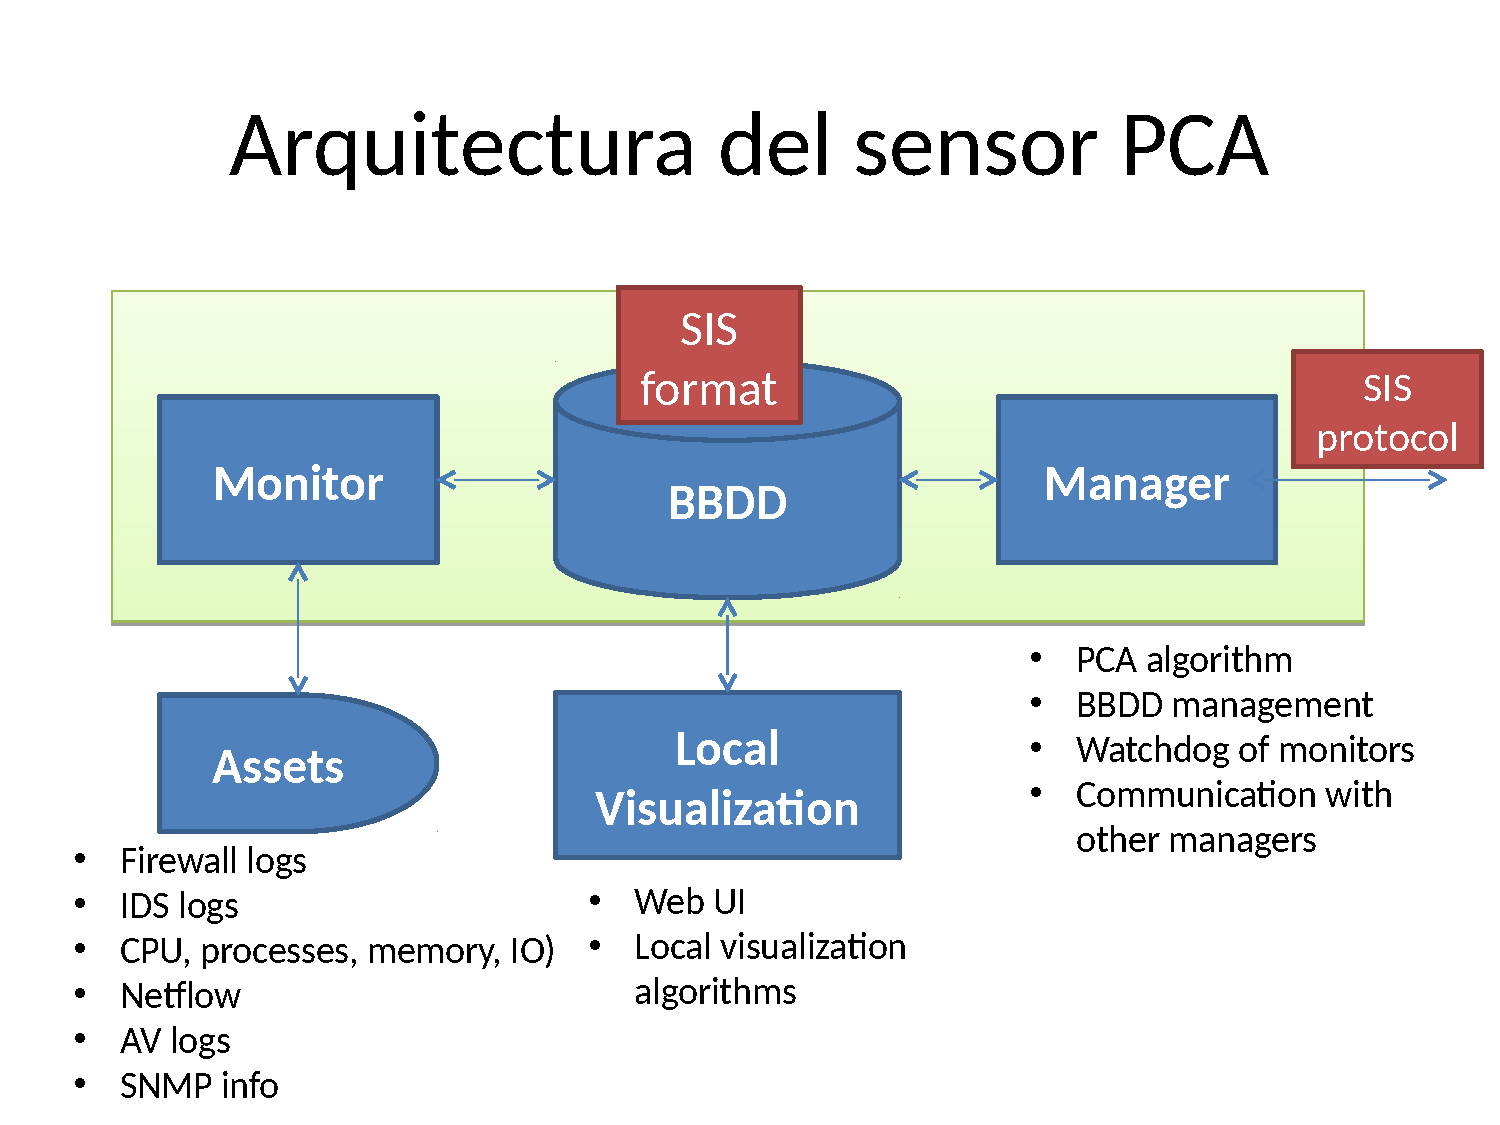
\includegraphics[scale=0.5]{diagramas/Especificaciones.pdf}}
  \caption{Arquitectura interna del software}
\end{figure}

En el esquema podemos ver toda la arquitectura que tendría una sonda para el proyecto VERITAS, aunque el ámbito de éste proyecto no se engloba en su totalidad, sino en unas partes en concreto del esquema que en el siguiente punto se explicarán en detalle. Puntualizar que la interacción de la sonda con la fuente de seguridad es independiente de la interacción base de datos con la visualización de los datos. Si bien se hace uso del mismo ORM, proporcionado por el framework Django, estos se ejecutan por separado a la hora de procesar las fuentes.

\section{Diseño del software de cada módulo}

\subsubsection{Assets}

\begin{figure}[H]
  \hspace*{0.65in}{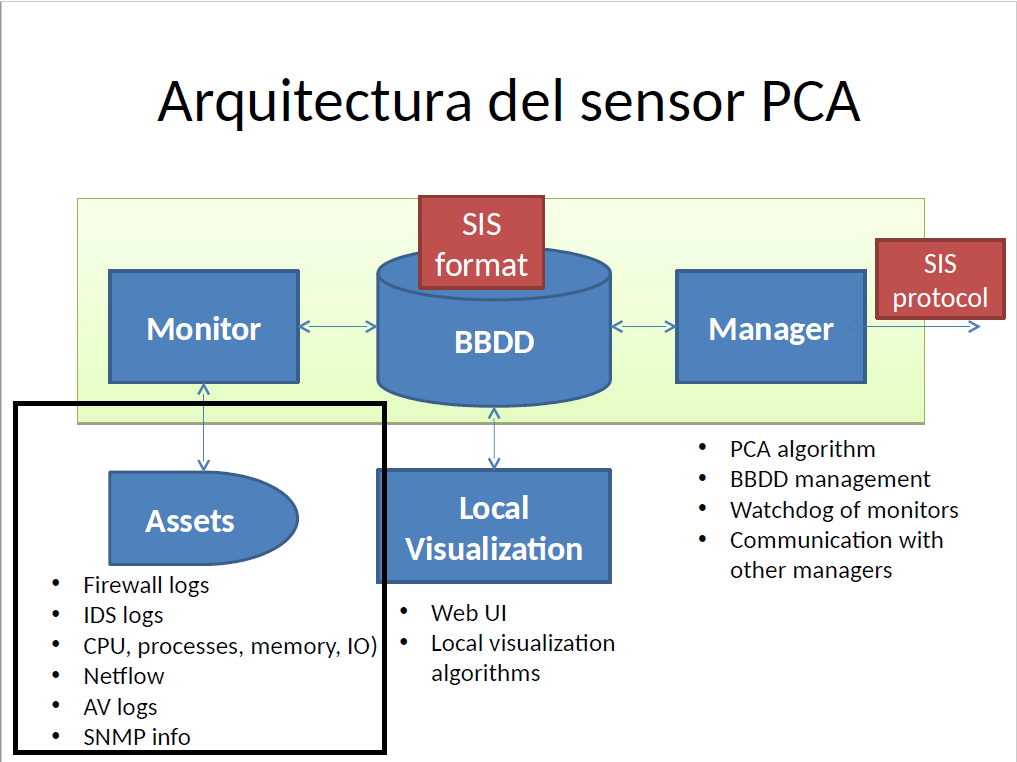
\includegraphics[scale=0.5]{diagramas/assets.png}}
  \caption{Arquitectura: Assets}
\end{figure}

En esta sección de la arquitectura es dónde se define la parte de las fuentes de seguridad que se van a gestionar desde la sonda, es decir, implementar, recolección y pasar el control final a su clase superior: Monitor. La jerarquía de clases sería de la siguiente manera:\\
\newpage
\begin{figure}
  \hspace*{0.05in}{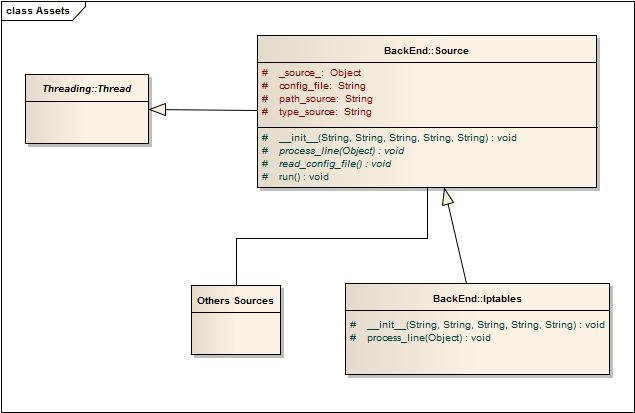
\includegraphics[scale=0.7]{diagramas/diagrama-assets.jpg}}
  \caption{Diagrama de clases: Assets}
\end{figure}

La clase base que sería Source, hereda del comportamiento de la clase Thread (de la biblioteca threading de Python) y a su vez toda fuente de seguridad que se decida implementar heredará de ella los métodos previstos.\\
\newpage

\subsubsection{Monitor}

\begin{figure}[H]
  \hspace*{0.65in}{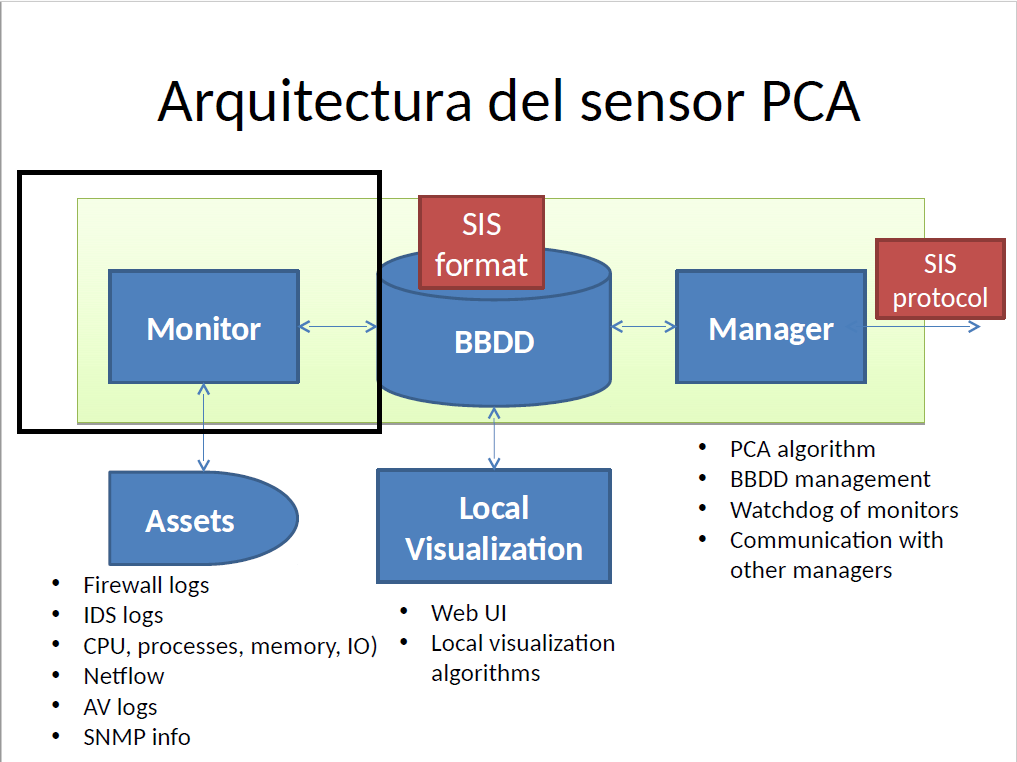
\includegraphics[scale=0.5]{diagramas/monitor.png}}
  \caption{Arquitectura: Monitor}
\end{figure}

En esta sección de la arquitectura es donde se define la parte del control y ejecución (hilos) de las fuentes de seguridad implementadas. A su vez, estas pasan dicha información a la base de datos usando el modelo ORM del framework Django. La jerarquía de clases sería de la siguiente manera: \\

\begin{figure}[H]
  \hspace*{-0.25in}{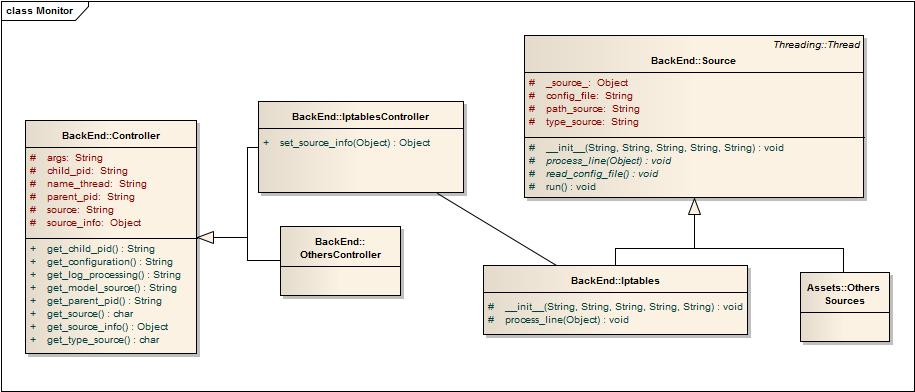
\includegraphics[scale=0.525]{diagramas/diagrama-monitor.jpg}}
  \caption{Diagrama de clases: Assets}
\end{figure}

Nuestra arquitectura monitor se representa con la clase Controller que se encarga de dotar de funcionalidad de ejecución de la fuente (hilo) para unos determinados parámetros de configuración.

\subsubsection{BBDD}

\begin{figure}[H]
  \hspace*{0.65in}{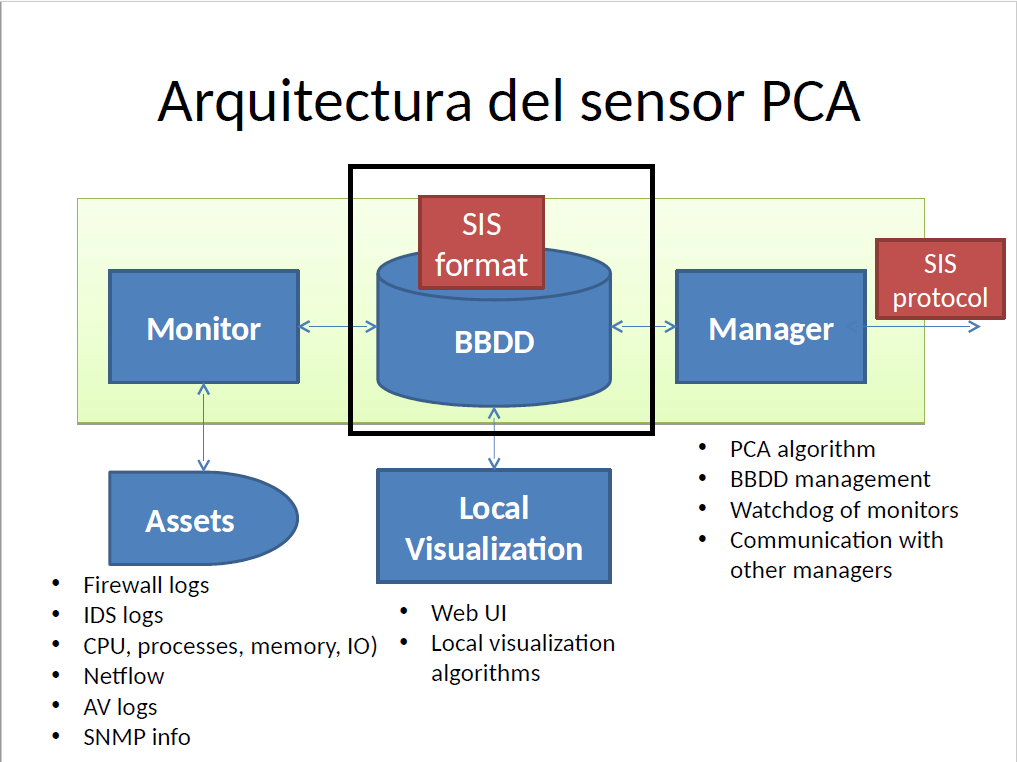
\includegraphics[scale=0.5]{diagramas/bbdd.png}}
  \caption{Arquitectura: Monitor}
\end{figure}

En esta sección de la arquitectura es dónde se define la parte de la interacción con la base de datos y que tablas (clases del modelo ORM) se han definido y con que relaciones. La jerarquía de clases sería de la siguiente manera: \\
\newpage
\begin{figure}[H]
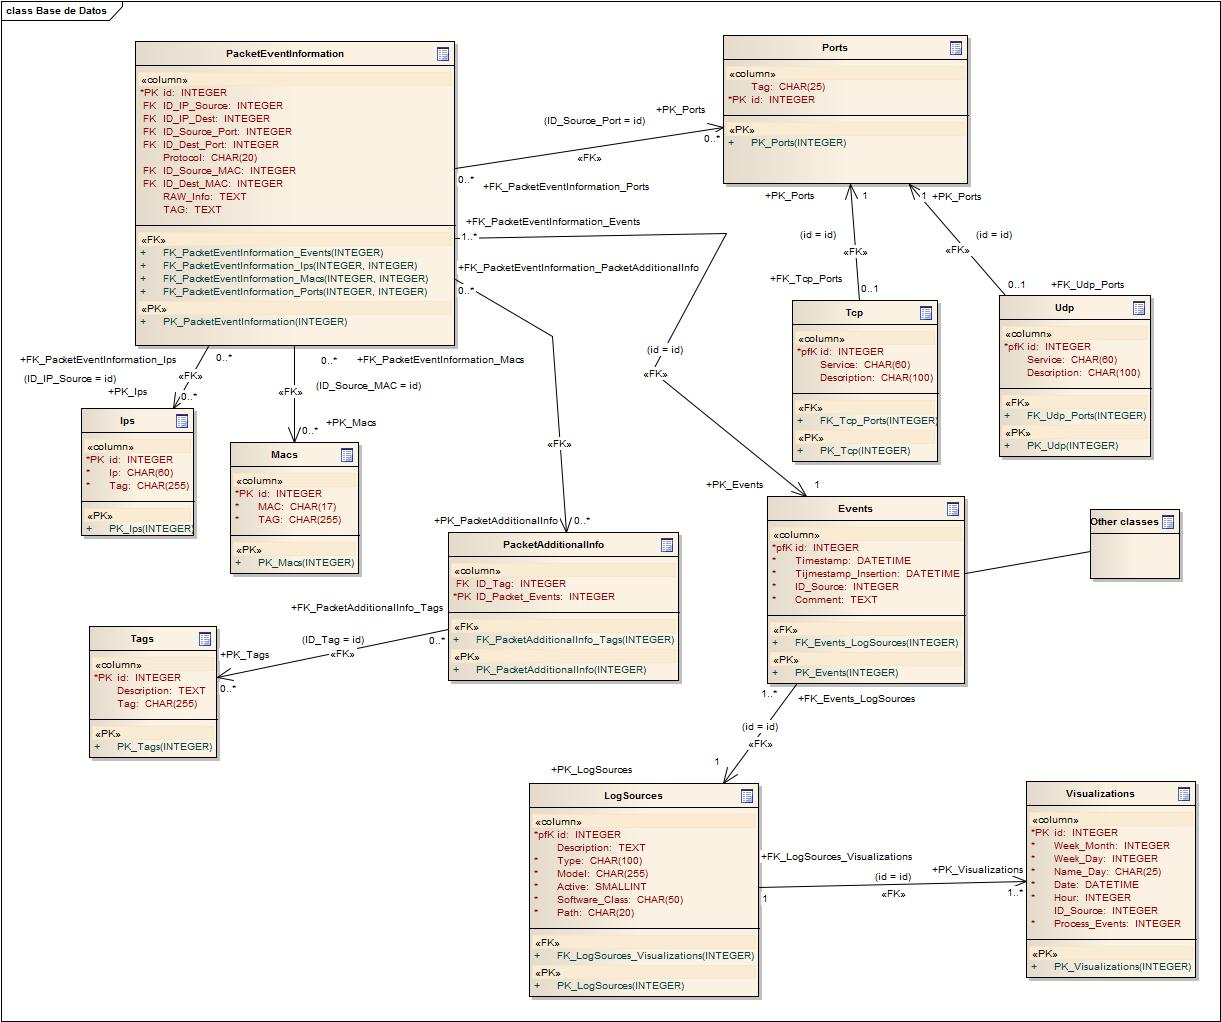
\includegraphics[scale=.35]{diagramas/bd.jpg}
\caption{Diagrama de clases para la BD (usando ORM)}
\end{figure}

La clase o tabla que contendrá el peso de toda la jerarquía de base de datos, será \textbf{PacketEventsInformation}. Esta tabla sólo contendrá referencias externas o ``foreign keys'' a cada tabla que haga participe en su definición, es decir:
\begin{itemize}
\item Ips
\item Macs
\item Ports
\item Events
\item PacketAdditionalInfo
\end{itemize}

Como podemos observar en el diagrama anterior, por ejemplo, para la clase PacketEventInformation, tenemos su traducción a formato ORM del motor proporcionado por Django:

\begin{figure}[H]
\lstinputlisting{trozos-codigo/codigo-8.py}
\caption{Ejemplo de clase ORM, en concreto PacketEventsInformation}
\end{figure}

El formato normalizado de la base de datos para visualizar dicha información será mediante JSON, ya que para hacer uso de la información la implementación consumirá dichos datos de la api que se proporciona con la aplicación.\\

\newpage
\subsubsection{Visualizations}

\begin{figure}[H]
  \hspace*{0.65in}{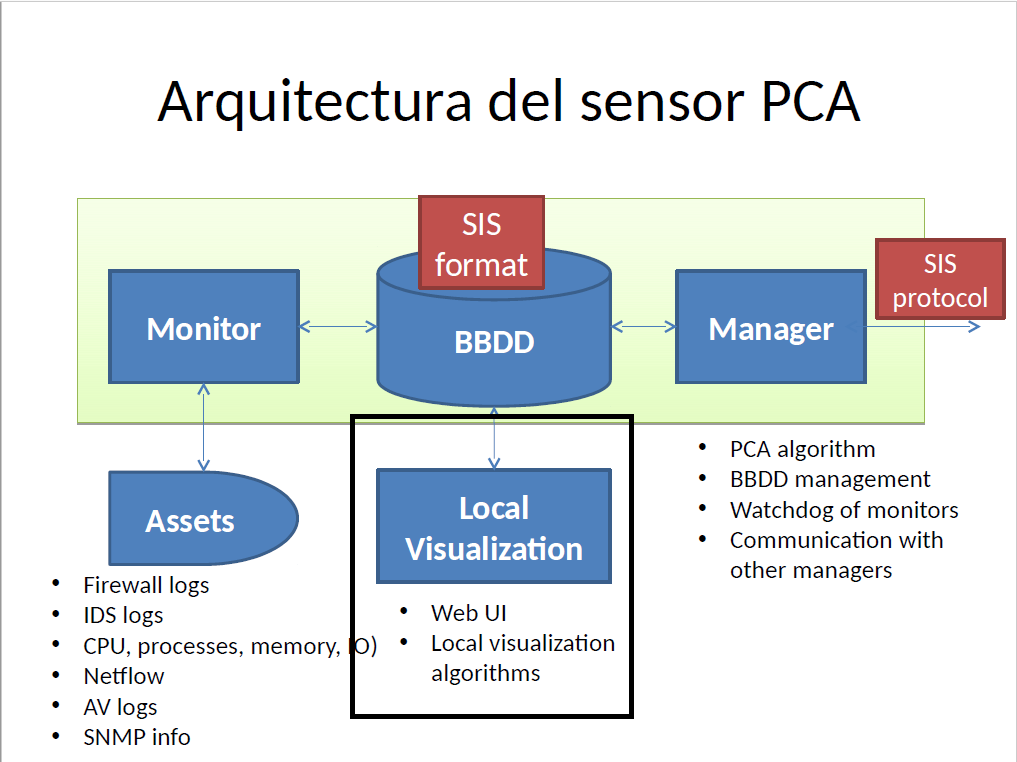
\includegraphics[scale=0.5]{diagramas/visualization.png}}
  \caption{Arquitectura: Visualizaciones}
\end{figure}

En esta seccción de la arquitectura es donde se define la parte de la interacción con la base de datos y la visualización de los datos en la interfaz web. La jerarquía de clases sería de la siguiente manera: \\

\begin{figure}[H]
  \hspace*{0.5in}{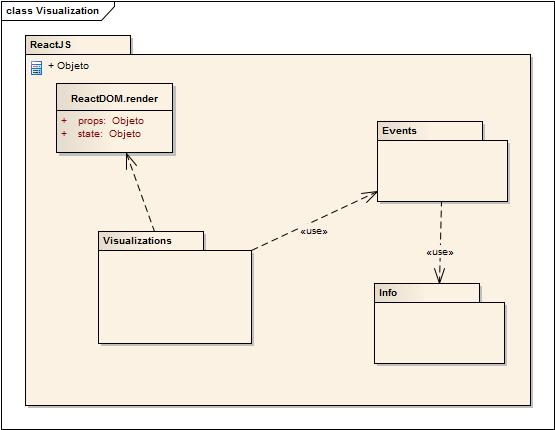
\includegraphics[scale=0.65]{diagramas/visualization.jpg}}
  \caption{Clase Visualization para el paquete ReactJS}
\end{figure}

\begin{figure}[H]
  \hspace*{0.75in}{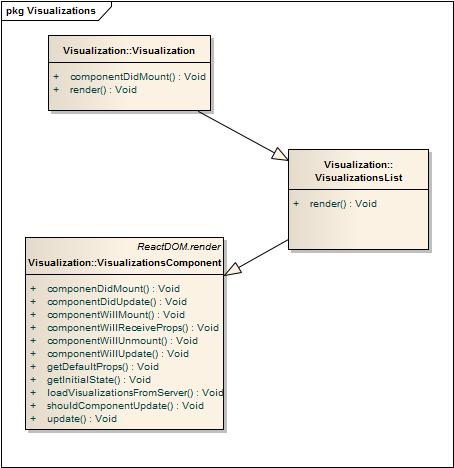
\includegraphics[scale=0.65]{diagramas/visualizations-visualizations.jpg}}
  \caption{Paquete Visualizations}
\end{figure}

\begin{figure}[H]
  \hspace*{0.75in}{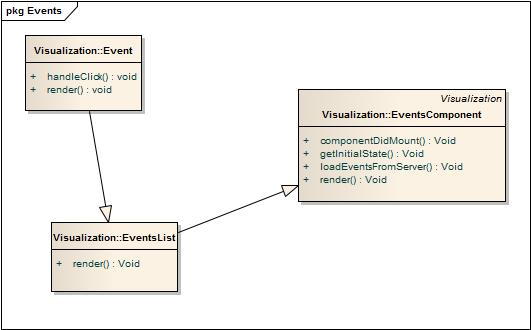
\includegraphics[scale=0.65]{diagramas/visualizations-events.jpg}}
  \caption{Paquete Events}
\end{figure}

\begin{figure}[H]
  \hspace*{2.15in}{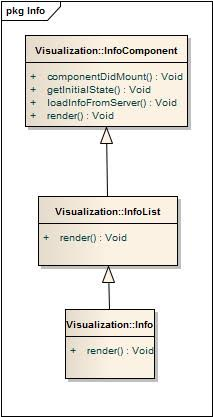
\includegraphics[scale=0.65]{diagramas/visualizations-info.jpg}}
  \caption{Paquete Info}
\end{figure}
\pagebreak
\section{Diagramas de Secuencia - Operaciones}

En esta sección vamos a describir los diagramas de secuencia de operaciones tales como:

\begin{itemize}
\item Ejecución principal de la sonda.
\item Ejecución principal del servidor web que sirve los datos a la interfaz web.
\end{itemize}

Ahora definiremos la parte de diagramas de secuencias para la interacción entre el usuario y el procesamiento de fuentes (Back); y el usuario y la visualización de los datos en la web de la aplicación (Front).\\
\newpage

\subsection{Flujo de ejecución de la aplicación: BackEnd}
\begin{figure}[H]
\vspace*{-.5in}{\hspace*{-.55in}{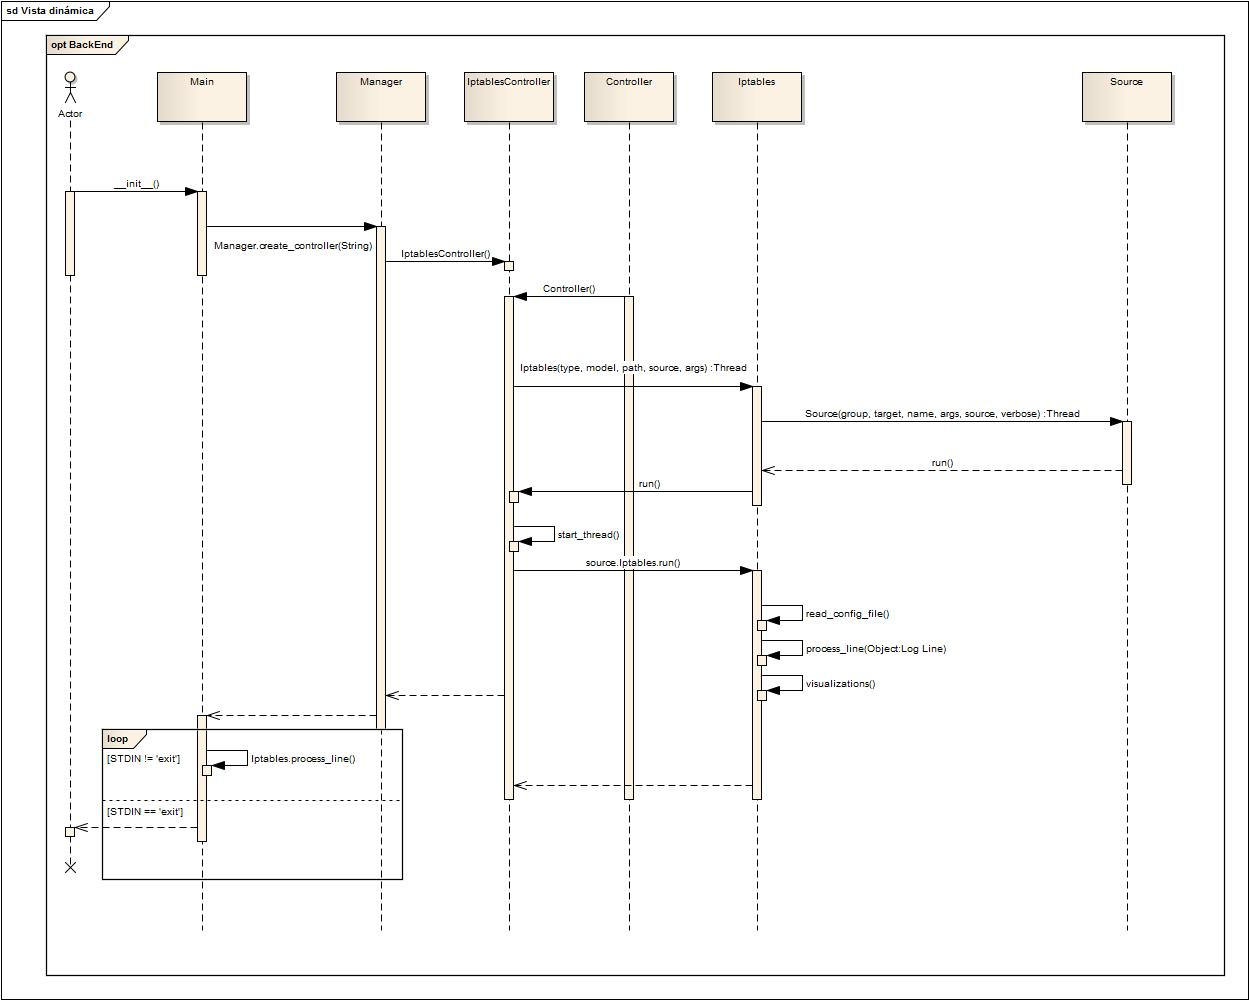
\includegraphics[scale=.5,angle=270]{diagramas/secuencia-back.jpg}}}
\caption{Diagrama de Secuencia para la parte BackEnd}
\end{figure}

\subsection{Flujo de ejecución de la aplicación: FrontEnd}

\begin{figure}[H]
\vspace*{-.1in}{\hspace*{.75in}{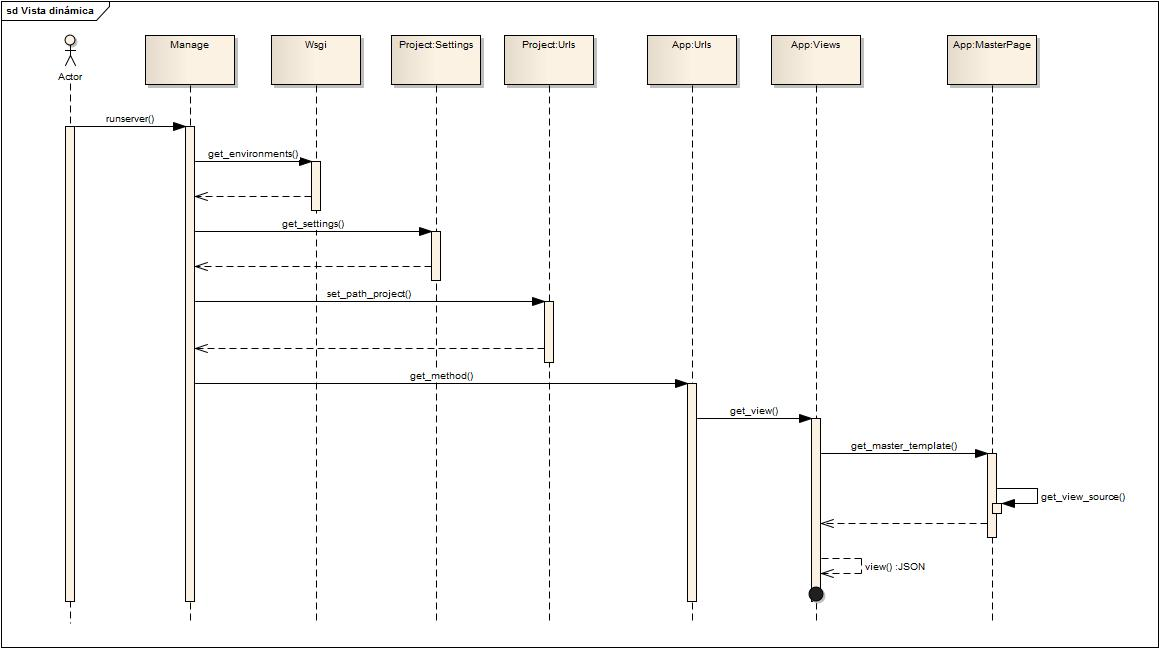
\includegraphics[scale=.5,angle=270]{diagramas/secuencia-front.jpg}}}
\caption{Diagrama de Secuencia para la parte FrontEnd}
\end{figure}

\section{Diseño de la vista}

\subsection{Flujo de interacción de la vista principal}

\begin{figure}[H]
\vspace*{-.1in}{\hspace*{.35in}{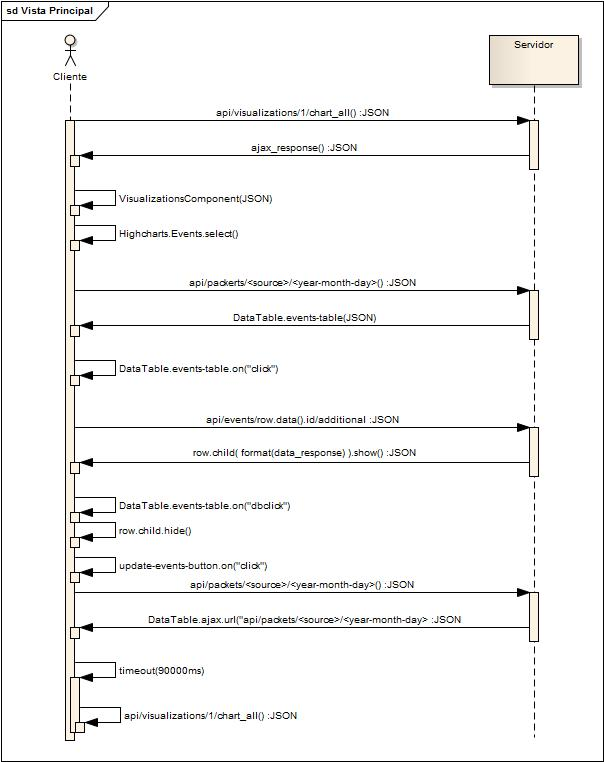
\includegraphics[scale=.7]{diagramas/vista-principal.jpg}}}
\caption{Diagrama de Secuencia para la vista principal}
\end{figure}

\subsection{Flujo de interacción de la vista de eventos en tiempo real}

\begin{figure}[H]
\vspace*{-.1in}{\hspace*{.65in}{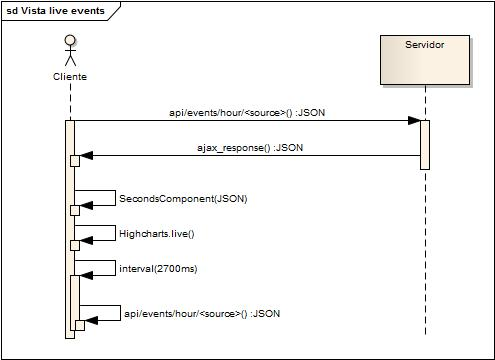
\includegraphics[scale=.7]{diagramas/vista-live-events.jpg}}}
\caption{Diagrama de Secuencia para la vista de eventos en tiempo real}
\end{figure}

\subsection{Flujo de interacción de la vista de estadísticas de los paquetes}

\begin{figure}[H]
\vspace*{-.1in}{\hspace*{.75in}{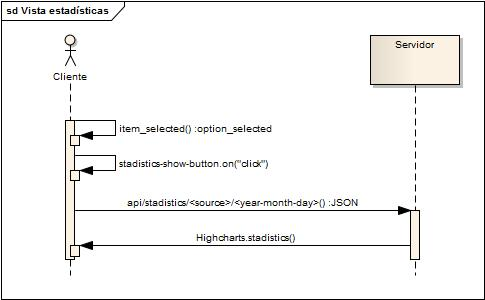
\includegraphics[scale=.7]{diagramas/vista-estadisticas.jpg}}}
\caption{Diagrama de Secuencia para la vista de estadísticas de los paquetes}
\end{figure}

Estos han sido los diagramas de secuencia o interacción que podrá tener la parte de la web con el usuario. Ahora se mostrarán algunas capturas de la parte visual (web) que finalmente se ha obtenido:

\subsubsection{Vista Principal}

\begin{figure}[H]
\vspace*{-.5in}{\hspace*{.55in}{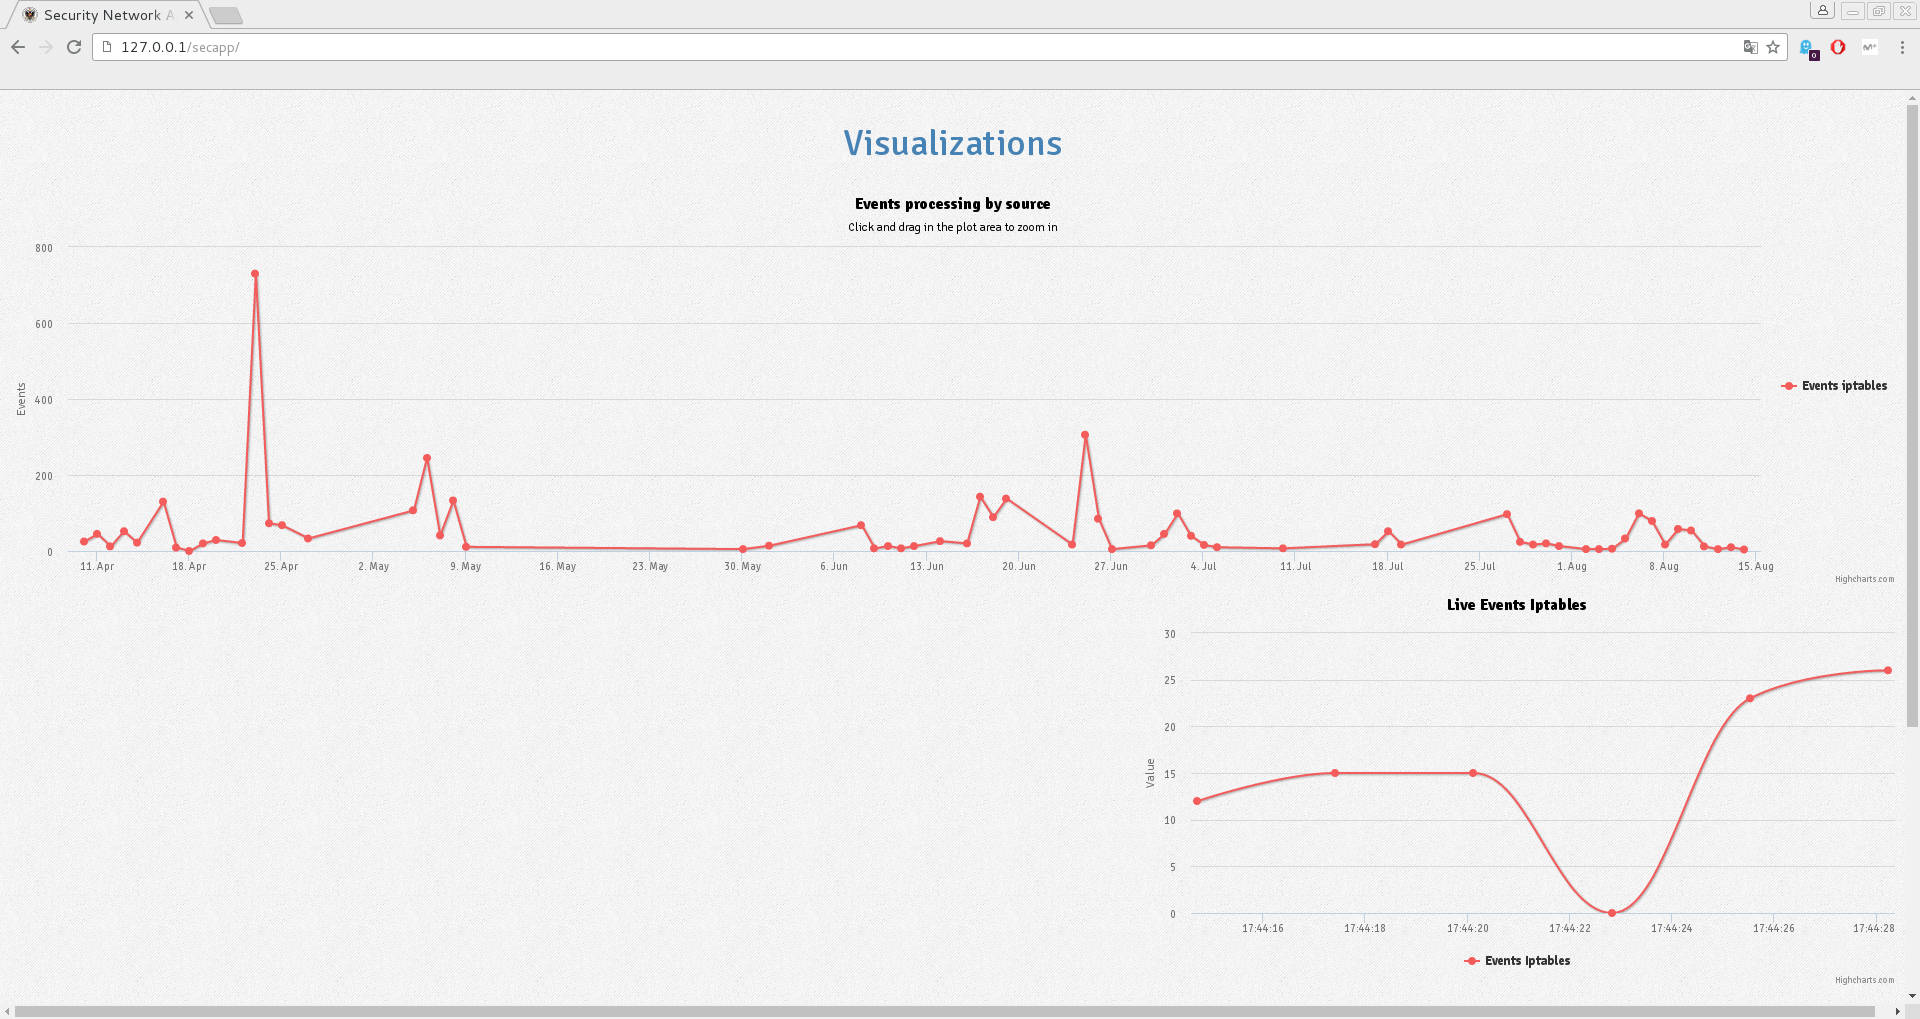
\includegraphics[scale=.32,angle=270]{diagramas/web_2.png}}}
\caption{Vista principal de la Web}
\end{figure}

\subsubsection{Vista con información de los eventos}

\begin{figure}[H]
\vspace*{.2in}{\hspace*{.55in}{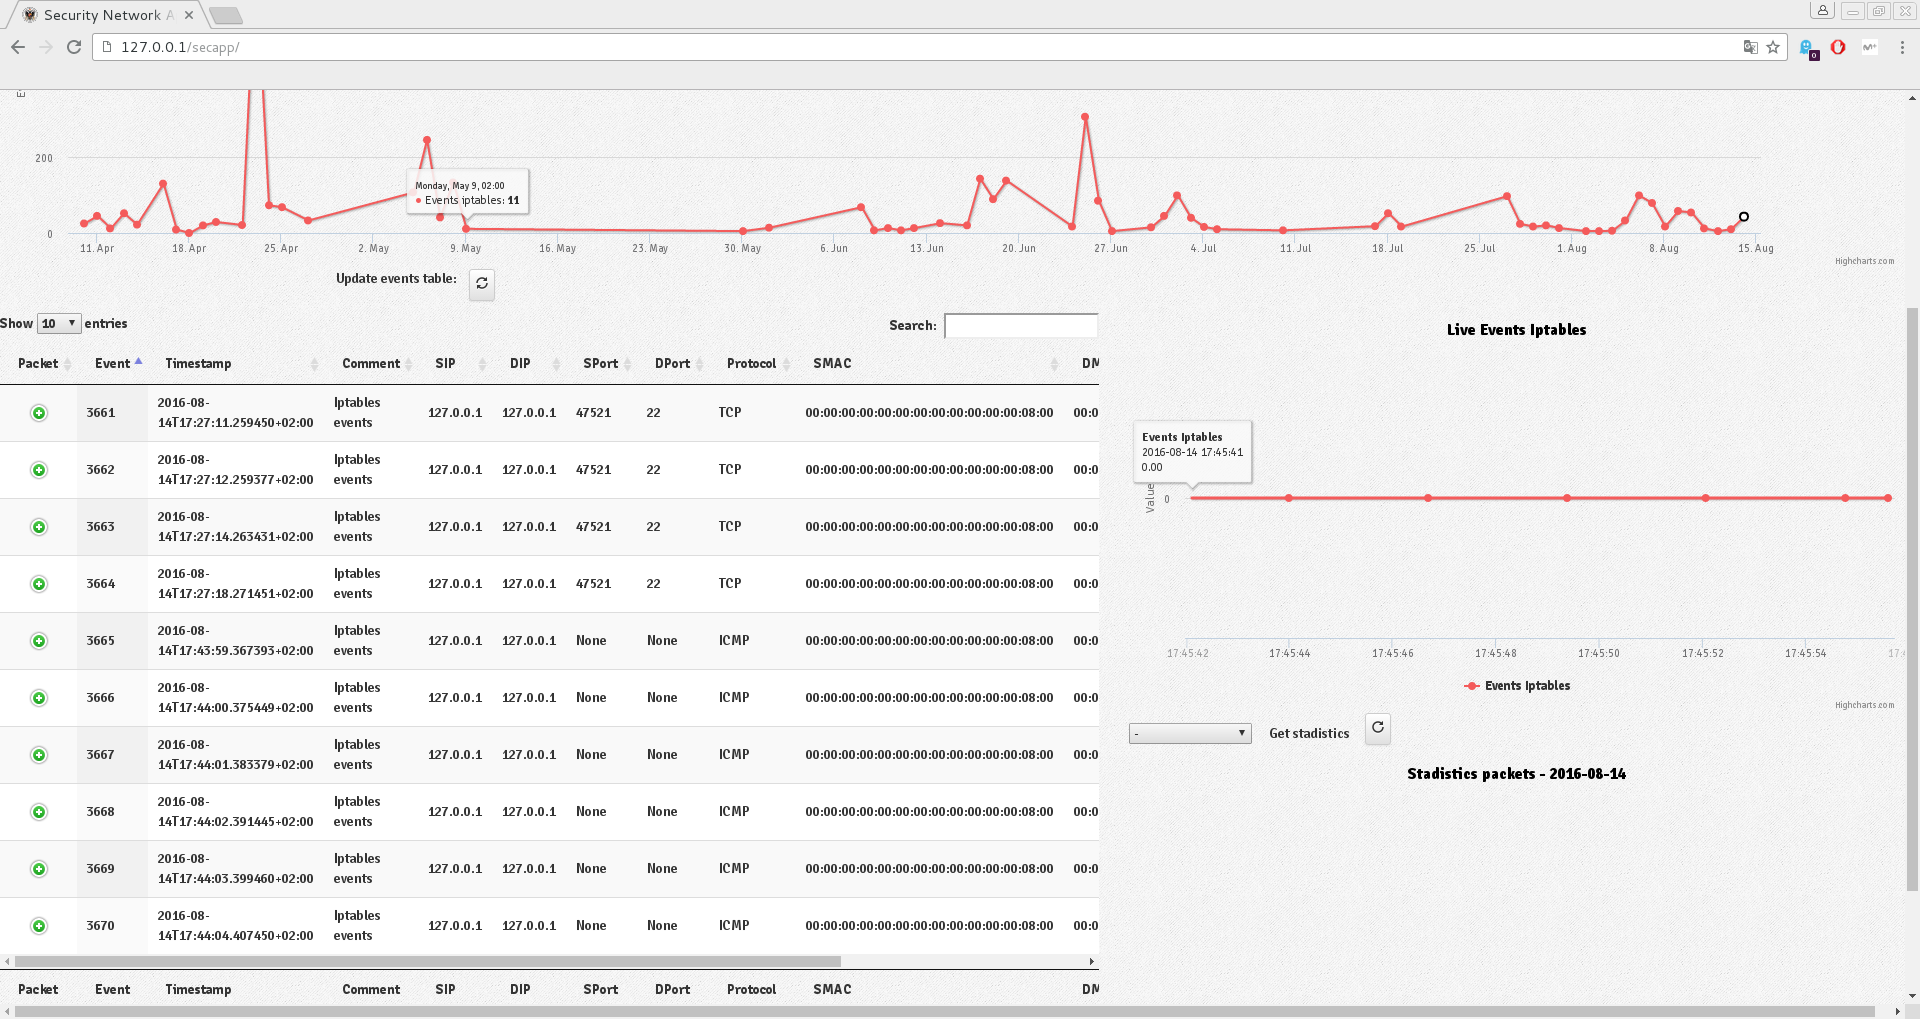
\includegraphics[scale=.32,angle=270]{diagramas/web_3.png}}}
\caption{Vista principal con la información de eventos del día seleccionado}
\end{figure}

\subsubsection{Vista con la información adicional por evento}

\begin{figure}[H]
\vspace*{.2in}{\hspace*{.55in}{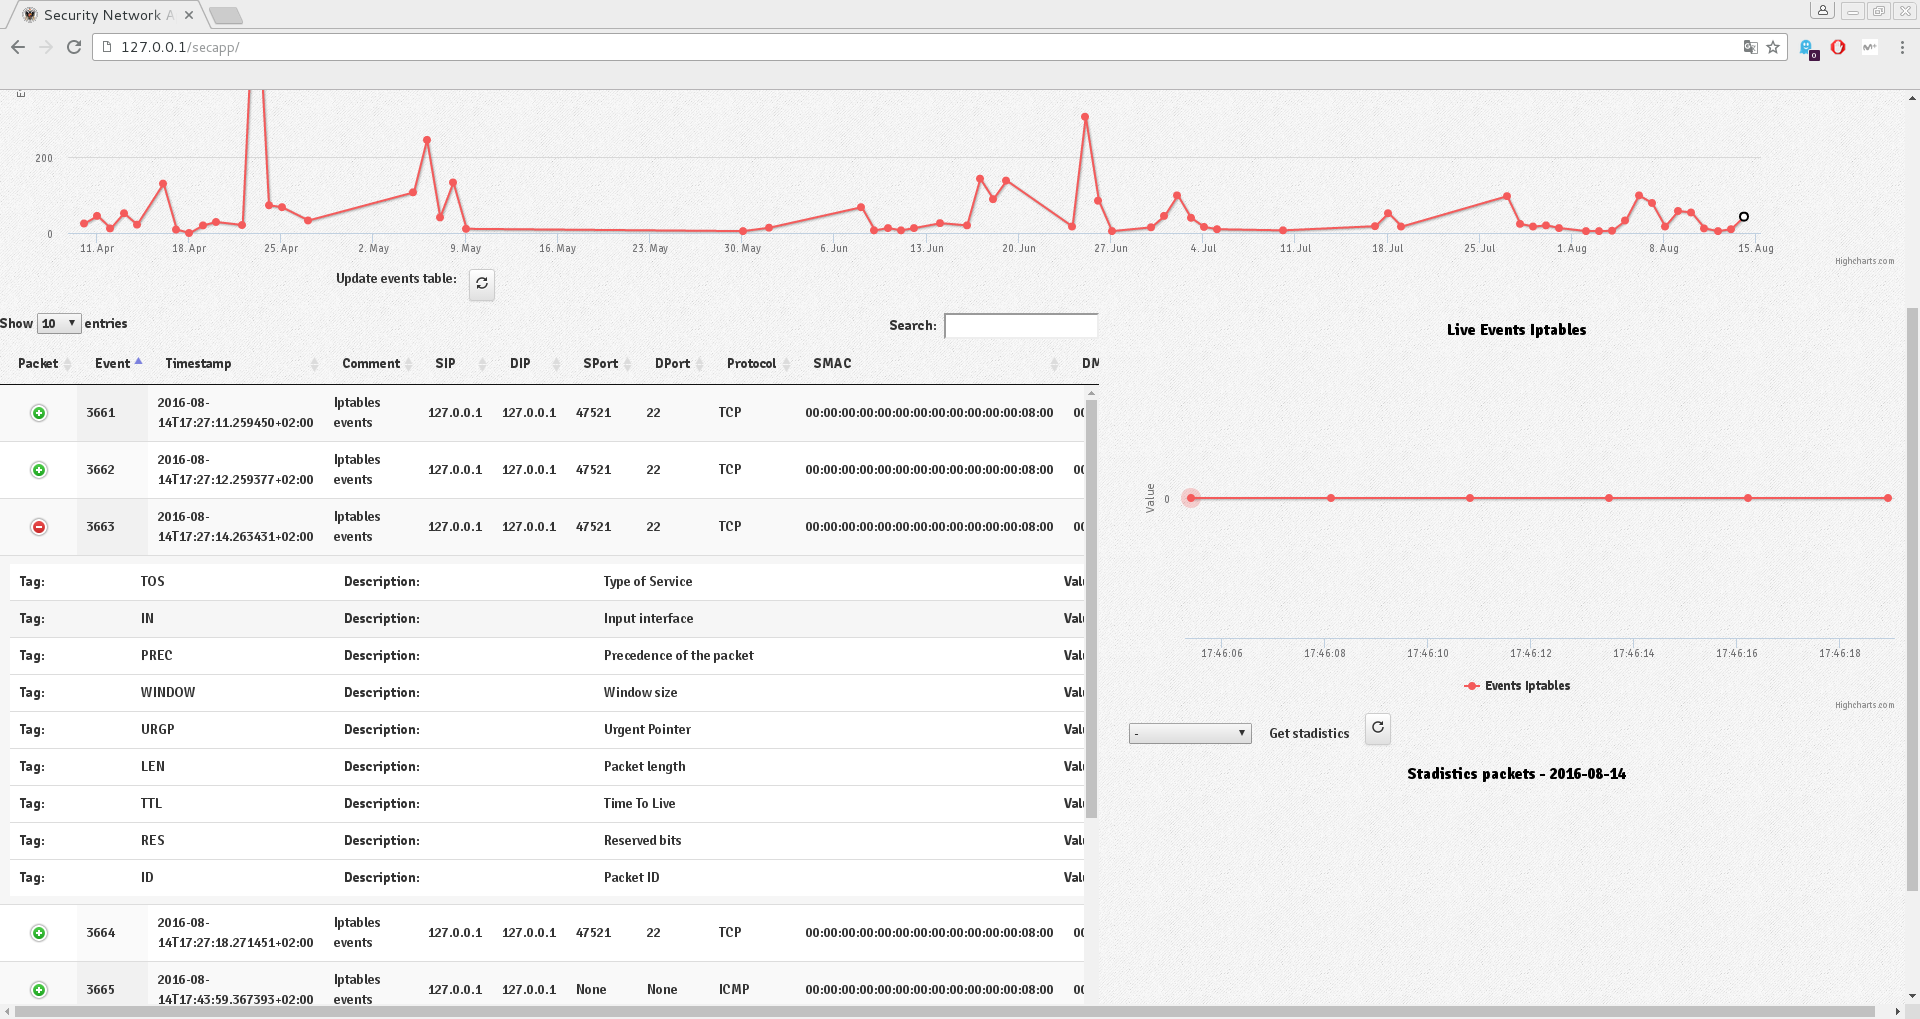
\includegraphics[scale=.32,angle=270]{diagramas/web_4.png}}}
\caption{Vista principal con la información adicional por cada evento seleccionado}
\end{figure}

\subsubsection{Vista con las estadísticas del día seleccionado}

\begin{figure}[H]
\vspace*{.2in}{\hspace*{.55in}{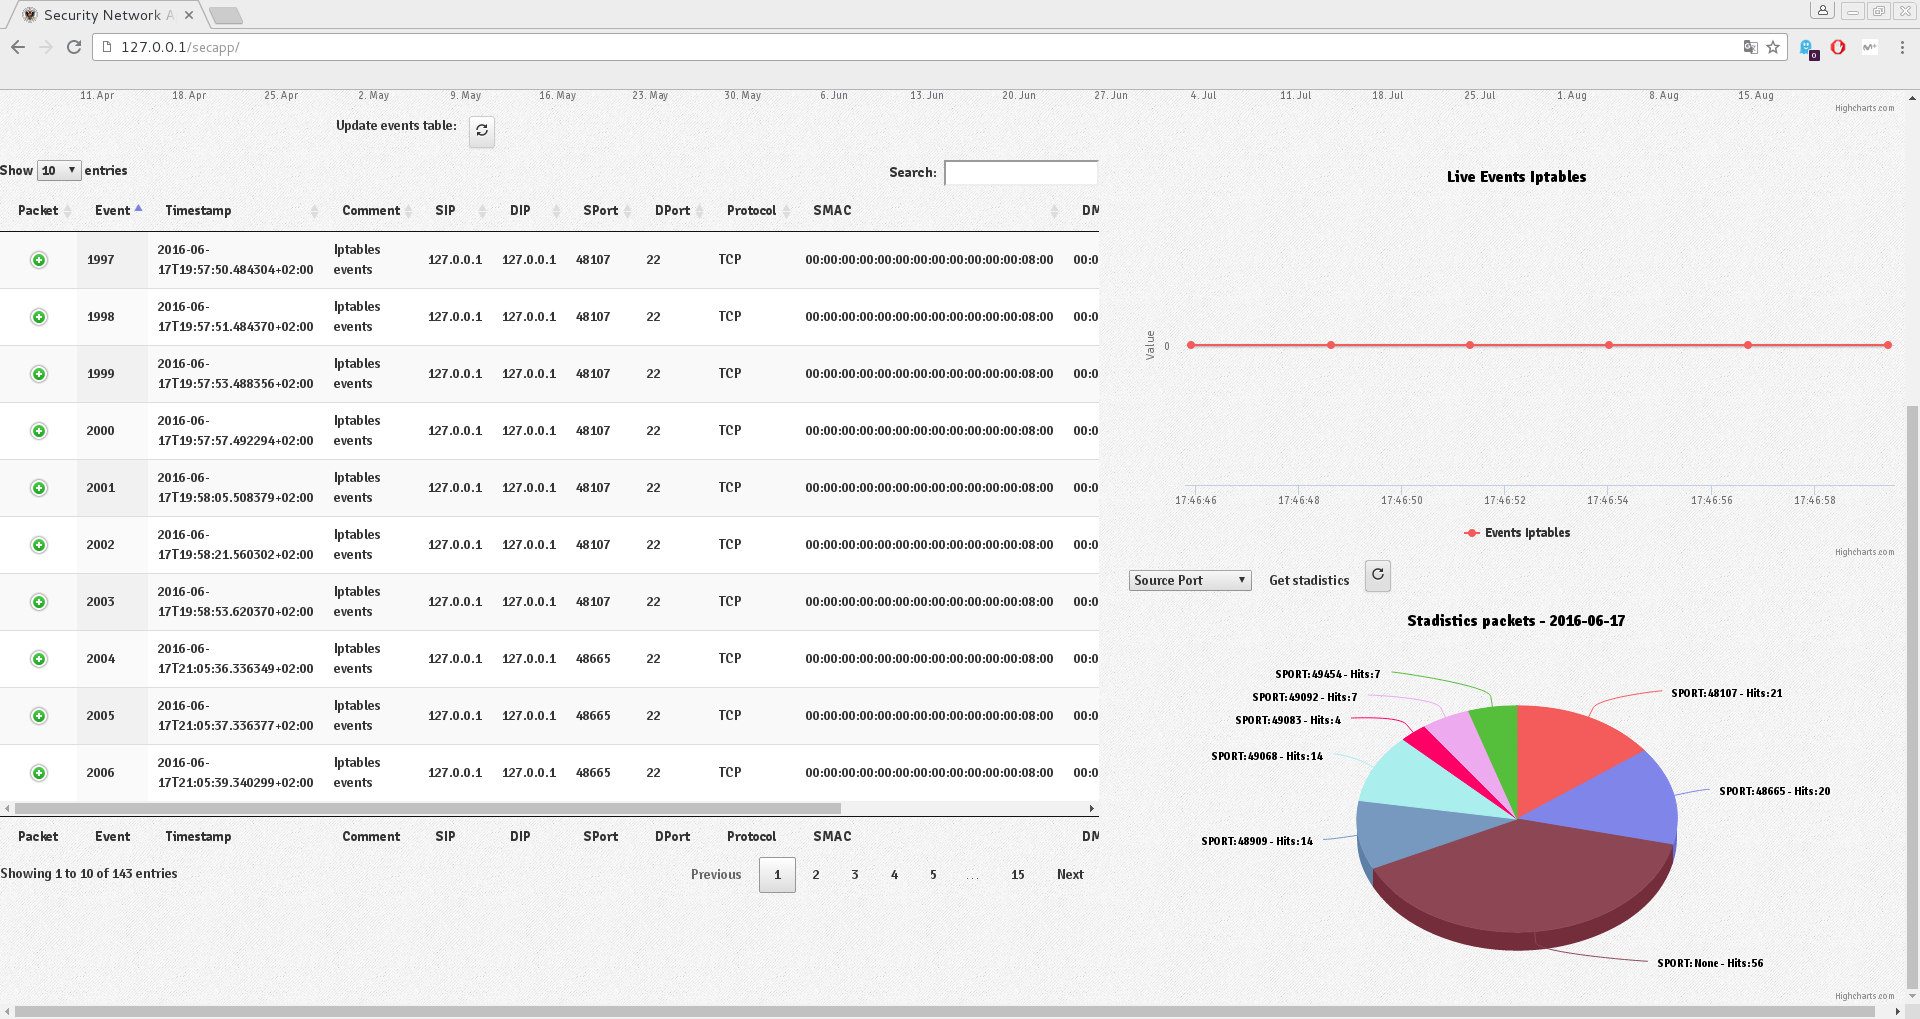
\includegraphics[scale=.32,angle=270]{diagramas/web_5.png}}}
\caption{Vista principal con las estadísticas de los eventos del día seleccionado}
\end{figure}
